\subsection{Maquinas de cambios}
	\label{sec:signal_switches}
	
    % Autoridad > derecho limitado a una porcion
    % Claridad > autoridad no ambigua
    % Anticipacion > avisar con antelacion
    % Granularidad > rutas cortas y funcionales
    % Terminalidad > avisar fin de via
    % Infraestructura > avisar de infraestructura
    % No bloqueo > circulacion fluida
    
    En la Sección \ref{sec:switches} definimos la clase switch que modela a las máquinas de cambios. Las máquinas de cambios son de los elementos ferroviarios mas críticos de la red. Por lo tanto, se deberá aplicar al principio de infraestructura ($P_6$) a cada una de sus entradas. Además, las máquinas de cambios actúan como una frontera entre las ramas principales de la red, donde se circula a mayor velocidad, y las ramas secundarias, donde se circula a una velocidad menor. Esto divide las rutas en dos o mas rutas, aplicando el principio de autoridad ($P_1$) y granularidad ($P_4$). Finalmente, por el principio de no bloqueo ($P_7$), será necesario generar señales de diferente tipo para las ramas principales y las secundarias, priorizando las primeras. Esto puede cumplirse si otorgamos señales de circulación de tres o mas aspectos a la rama principal y señales de maniobra para utilizar una rama secundaria como salida o entrada de la red.
    
    En el Algoritmo \ref{alg:SW} definimos al punto de acceso de inicio como la vía desde la cual la trayectoria de la formación se bifurca, para lo cual se genera una señal de circulación para continuar por la rama principal y una señal de maniobra para acceder a la rama secundaria. Además, se añade una señal de circulación en la rama principal y una señal de maniobra en la rama secundaria, ambas en sentido contrario, para poder retornar al punto de inicio. 
    
    \begin{algorithm}[H]
        \caption{Algoritmo de generación de señalamiento para Switches}\label{alg:SW}
        \DontPrintSemicolon
        %\SetAlgoLined
        \SetNoFillComment
        \LinesNotNumbered 
        \For { Switch in Switches }
        {
            \tcc{All signals must point to switch}
            \Switch{ Switch.Type }
            {
                \Case{Start}
                {
                    [Signals] $\gets$ ADD circulation signal\;
                    [Signals] $\gets$ ADD maneuver signal\;
                }
                \Case{Continue branch}
                {
                    [Signals] $\gets$ ADD circulation signal\;
                }
                \Case{Detour branch}
                {
                    [Signals] $\gets$ ADD maneuver signal\;
                }
            }   
        }
        \KwResult{[Signals]} 
    \end{algorithm}

    Aplicando el Algoritmo \ref{alg:SW} a un sistema de vías que se bifurcan obtenemos el resultado ilustrado en la Figura \ref{fig:signal_swithces}. Se asumieron que ambas vías son bidireccionales. En caso contrario, si el sentido de circulación es únicamente de bifurcación, las señales de retorno S02 y S03 no son necesarias. Si el sentido de circulación fuese de derecha a izquierda, las señales de inicio S01 no son necesarias.
    
    \begin{figure}[H]
        \centering
        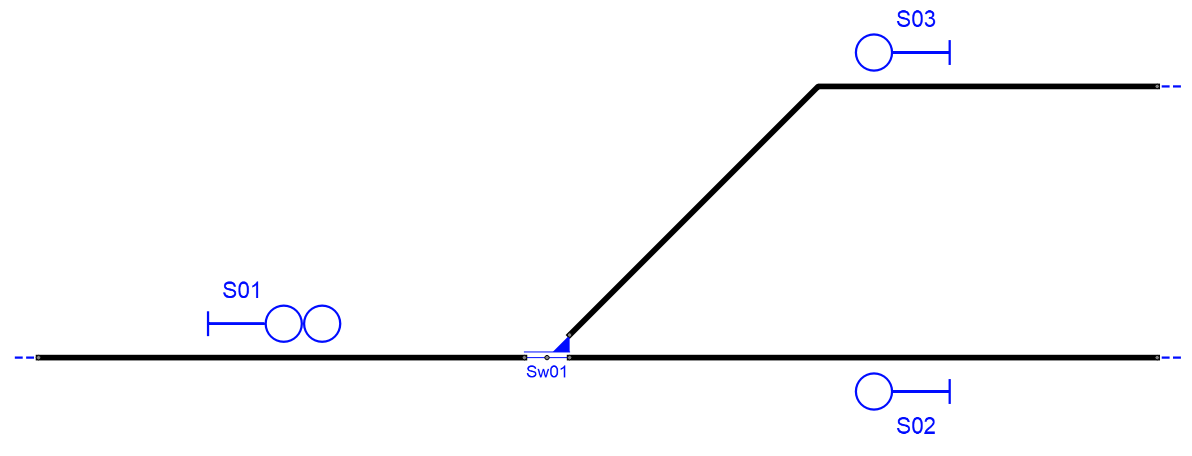
\includegraphics[width=1\textwidth]{Figuras/switches.PNG}
        \centering\caption{Señalamiento generado para cambios de vías.}
        \label{fig:signal_swithces}
    \end{figure}
    
    Una formación que circule de izquierda a derecha deberá detenerse antes de la señal S01. El aspecto mas cercano al poste de la señal S01 indicará si la formación puede circular por la vía principal, como se explicó en la Sección \ref{sec:signals}, previa confirmación por parte del sistema de enclavamiento de que el cambio Sw01 se encuentra en posición normal. De la misma forma, el sistema de enclavamiento confirmará que el cambio Sw01 se encuentra en posición reverso previo a habilitar la circulación por la vía secundaria mediante el aspecto mas alejado al poste de la señal S01.

    Una formación circulando de derecha a izquierda hará uso de las señales S02 y S03 si se encuentran en las vías principal o secundaria respectivamente. Las señales se habilitarán si el sistema de enclavamientos confirma que el cambio Sw01 se encuentra en la posición normal o reverso respectivamente y si no hay formaciones ocupando la vía de inicio donde se encuentra la señal S01, continuando su marcha hasta la próxima señal disponible, fuera del alcance de lo ilustrado en la Figura \ref{fig:signal_swithces}.    